\chapter{Boyle's Law}

\section{Aim}
To find out how the volume of a gas relates to its pressure at constant temperature

\section{Background Information}
In gasses, volume, pressure and temperature depend on one another. It is a bit difficult to study the variations of the three quantities at the same time. If one of the three variables is kept constant, the variations of the remaining two can be investigated. It is very important to find out how volume relates with pressure at constant temperature for a better understanding of gasses.

\section{Materials}
Glass tube, bicycle pump, Bourdon gauge, oil

\section{Procedure}
\begin{enumerate}
\item Trap a mass of air in the glass tube with oil and read the volume $V$ of the air and the corresponding pressure $P$ of the trapped air using the Bourdon gauge.
\item Connect the bicycle pump and gently increase the pressure $P$ of the air in the tube and record the corresponding volume $V$. See Figure \ref{fig:boyles-law-1}.
\item Obtain five more values of $P$ and the corresponding values of volume $V$ and tabulate your results.
\end{enumerate}

\begin{figure}[h!]
\centering
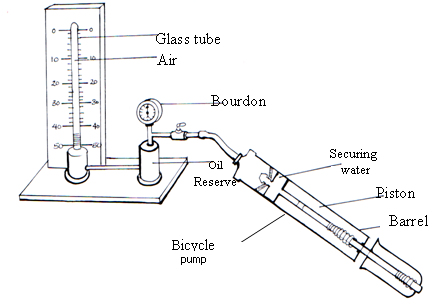
\includegraphics[width=10cm]{./img/boyles-law-1.png}
\caption{Boyle's Law practical setup}
\label{fig:boyles-law-1}
\end{figure}

\section{Safety Measure}
Pumping of the oil should be done slowly so as to avoid an increase in the temperature.

\section{Analysis and Interpretation}
\begin{enumerate}
\item Compute the values of $^1/_V$ and include them in the table.
\item Plot the graph of P against $^1/_V$.
\item What is the nature of the graph?
\item From the graph find the slope, what does it represent?
\end{enumerate}

\section{Conclusion}
From the results of this experiment what is the relationship between pressure and volume of a gas at constant temperature?

\section{Questions for Discussion}
\begin{enumerate}
\item Why in this experiment is it necessary to maintain the temperature of the air (gas)?
\item Suppose a graph of pressure against volume was plotted, what will be the nature of the graph?
\item Based on the results of this experiment, what could be a cause for high blood pressure in a person?
\end{enumerate}

\section{Reflection and Self Assessment}
\begin{enumerate}
\item What parts of this experiment were most and least interesting to you? Explain.
\item How can you use the results of this experiment in you daily life? 
\end{enumerate}